
%%%%%%%%%%%%%%%%%%%%%%%%%%%%%%%%%%%%%%%%%
% Tufte Essay
% LaTeX Template
% Version 2.0 (19/1/19)
%
% This template originates from:
% http://www.LaTeXTemplates.com
%
% Authors:
% The Tufte-LaTeX Developers (https://www.ctan.org/pkg/tufte-latex)
% Vel (vel@LaTeXTemplates.com)
%
% License:
% Apache License, version 2.0
%
%%%%%%%%%%%%%%%%%%%%%%%%%%%%%%%%%%%%%%%%%

%----------------------------------------------------------------------------------------
%	PACKAGES AND OTHER DOCUMENT CONFIGURATIONS
%----------------------------------------------------------------------------------------

\documentclass[a4paper]{tufte-handout} % Use A4 paper by default, remove 'a4paper' for US letter

\usepackage{graphics}
\usepackage{graphicx} % Required for including images
\setkeys{Gin}{width=\linewidth, totalheight=\textheight, keepaspectratio} % Default images settings

\usepackage{amsmath, amsfonts, amssymb, amsthm} % For math equations, theorems, symbols, etc
\usepackage{units} % Non-stacked fractions and better unit spacing
\usepackage{physics}
\usepackage{cancel}

\usepackage{booktabs} % Required for better horizontal rules in tables

% For newtcbtheorem
\usepackage[most]{tcolorbox}
\usepackage{cleveref}

\setlength{\marginparwidth}{0mm}
\setlength{\parskip}{1em}


%----------------------------------------------------------------------------------------
%	TITLE SECTION
%----------------------------------------------------------------------------------------

\title{Smart Materials\\ Problem set \#3: Shape memory effect}

\author{Francisco Vazquez-Tavares}

\date{\today} % Date, use \date{} for no date


%----------------------------------------------------------------------------------------
%	COMMANDS SECTION
%----------------------------------------------------------------------------------------

\newcommand{\hata}{\hat{a}}
\newcommand{\hatad}{\hat{a}^\dagger}
\newcommand{\QDi}{\hat{X}_1}
\newcommand{\QDj}{\hat{X}_2}

\newtcbtheorem[]{prob}{Problem}%
    {enhanced,
    colback = black!5, %white,
    colbacktitle = black!5,
    coltitle = black,
    boxrule = 0pt,
    frame hidden,
    borderline west = {0.5mm}{0.0mm}{black},
    fonttitle = \bfseries\sffamily,
    breakable,
    before skip = 3ex,
    after skip = 3ex
}{def}


%----------------------------------------------------------------------------------------

\begin{document}

\maketitle % Print the title section
\justifying

%----------------------------------------------------------------------------------------
%	ESSAY BODY
%----------------------------------------------------------------------------------------

\begin{prob}{~}{label1}
Assuming that the stress required to initiate martensitic transformation in a Nitinol wire increases linearly by 5 MPa for every 1°C increase in temperature, calculate the stress required to initiate martensitic transformation at 50°C. 
It is given that Nitinol undergoes martensitic transformation at a stress of 300 MPa at 30°C.
\end{prob}

\begin{prob}{~}{label2}
A SMA wire shows a stress plateau during martensitic transformation from 350 MPa to 400 MPa. 
The strain increases from 0.02 to 0.05 during this plateau. 
Calculate the approximate work done per unit volume during the martensitic transformation.
\end{prob}

\begin{prob}{~}{label3}
A Nitinol wire has a stress-induced martensitic transformation starting at 200 MPa at 30 °C and ending at 500 MPa. 
The transformation stress increases by 10 MPa/°C. 
If the wire is heated to 80 °C, determine the new stress required to start and complete the transformation. 
Calculate the stress required to start and complete the transformation at 80 °C.
\end{prob}

\begin{prob}{~}{label4}
The martensite start and finish temperatures (Ms and Mf), the austenite start and finish temperatures (As and Af) and the slopes of the variation of Ms and Mf with stress (T) i.e., CM and the slope of variation of As and Af with T, i.e., CA, of a shape memory material are as follows: Ms = 25 ◦C, Mf = 5 ◦C, As = 29 ◦C, Af = 51 ◦C, CA = 4.5 MPa/◦C, CM = 11.3 MPa/◦C. 
The elastic modulus of the material is 15 GPa and it has a recovery strain of 8\%. 
For this material compute the following: 
\begin{itemize}
    \item Calculate the martensitic fraction when the material is cooled to 20 °C from 25 °C in a zero-stress state.
    \item If the temperature is maintained at 25 °C, determine the martensitic fraction when a tensile stress of 100 MPa is applied to the wire.
    \item The wire is heated above Af = 51 ◦C, and then cooled under zero stress to 30 °C. Subsequently, it is subjected to loading to activate the shape memory effect, leading to complete phase transformation, starting from point a to point e (as illustrated in the Figure below).
\end{itemize}
Calculate the stress and strain values at points a, b, c, and d on the stress–strain diagram.
\end{prob}

\begin{figure}[ht!]
    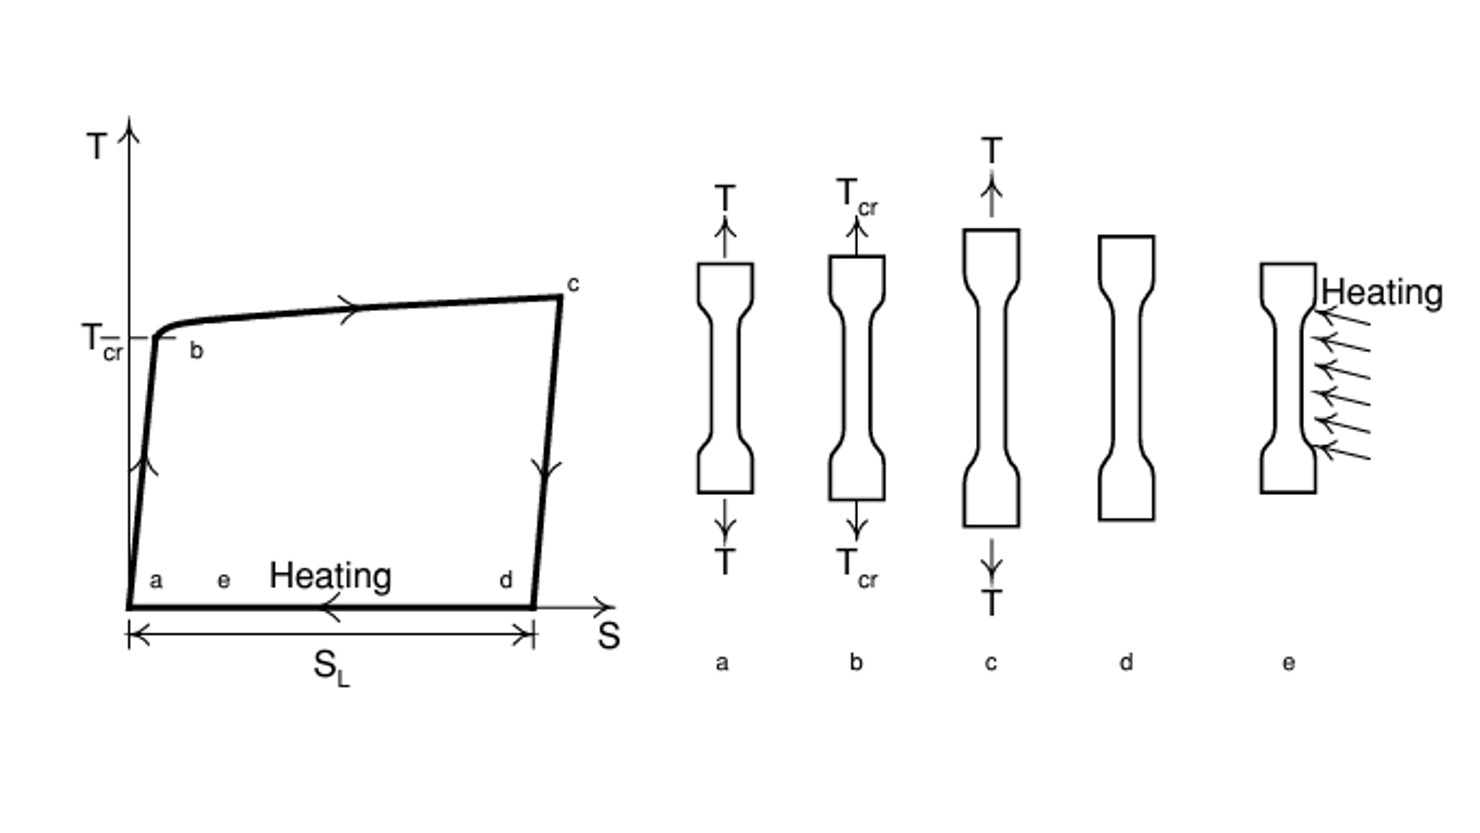
\includegraphics[width=0.9\textwidth]{imgs/SMAcurve.jpg}
    \caption{Strain-Stress curve}\label{fig:hmk2}
\end{figure}


\end{document}
